\paragraph{}En este proceso, el usuario administrador de centro puede crear,
consultar, modificar o borrar usuarios asesores de la aplicación.

\paragraph{}La figura \ref{diagramaNivel5-AdministrarAsesores-admCentro}
muestra el nivel de abstracción 5: Administrar Asesores (módulo Administrador
de centro).

  \begin{figure}[!ht]
    \begin{center}
      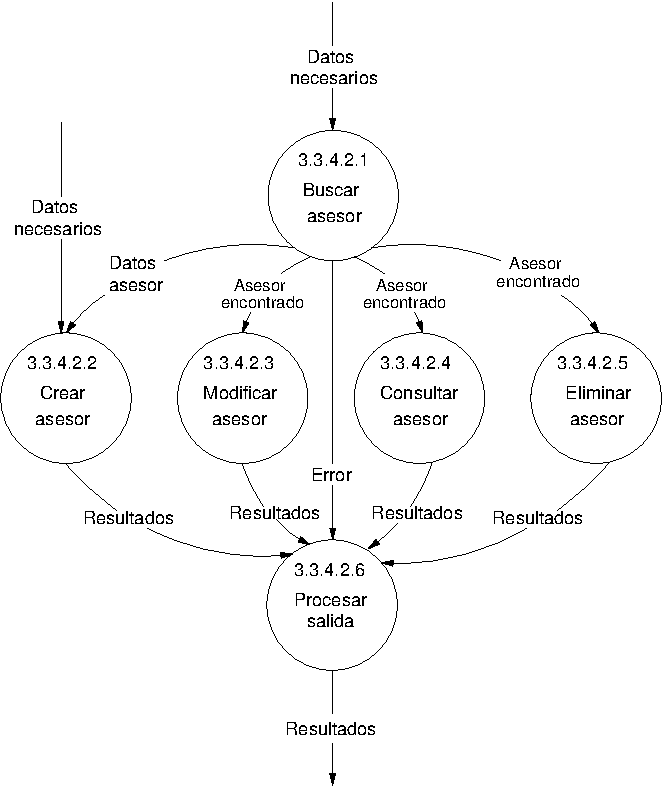
\includegraphics[]{08.Analisis_Funcional/8.2.DFDs/Niveles/Nivel5/AdministradorCentro/AdministrarUsuarios/AdministrarAsesores/Diagramas/nivel5-AdministrarAsesores.pdf}
      \caption{Nivel de abstracción 5: Administrar Asesores (módulo
      Administrador de centro).}
      \label{diagramaNivel5-AdministrarAsesores-admCentro}
    \end{center}
  \end{figure}
